\chapter{Лабораторная работа 6}

Целью лабораторной работы №6 является ознакомление с существующими методиками предварительной оценки параметров программного проекта и практическая оценка затрат на примере методики COCOMO (COnstructive COst MOdel --- конструктивная модель стоимости).

\section*{Методика конструктивной модели стоимости}

Конструктивная модель стоимости (англ. \textit{COnstructive COst MOdel}, \linebreak COCOMO) --- алгоритмическая модель оценки стоимости разработки программного обеспечения, разработанная Барри Боэмом.
Модель использует простую формулу регрессии с параметрами, определенными из данных, собранных по ряду проектов.

\begin{equation}
\textup{Трудозатраты} = c_1 \times EAF \times \textup{Размер}^{p_1},
\end{equation}

\begin{equation}
\textup{Время} = c_2 \times \textup{Трудозатраты}^{p_2},
\end{equation}

где:

Трудозатраты --- количество человеко-месяцев.

$c_1$ --- масштабирующий коэффициент.

EAF --- уточняющий фактор, характеризующий предметную область, персонал, среду и инструментарий, используемый для создания рабочих продуктов процесса.

Размер --- размер конечного продукта (кода, созданного человеком), измеряемый в исходных инструкциях (DSI, delivered source instructions), которые необходимы для реализации требуемой функциональной возможности.

$p_1$ --- показатель степени, характеризующий экономию при больших масштабах, присущую тому процессу, который используется для создания конечного продукта; в частности, способность процесса избегать непроизводительных видов деятельности (доработок, бюрократических проволочек,
накладных расходов на взаимодействие).

Время --- общее количество месяцев.

$c_2$ --- масштабирующий коэффициент для сроков исполнения.

$p_2$ --- показатель степени, который характеризует инерцию и распараллеливание, присущие управлению разработкой ПО.

Методика COCOMO может быть использована для построения модели, позволяющей исследовать зависимость трудоёмкости и времени разработки от типа проекта (обычный, промежуточный, встроенный), а также определить влияние на трудоёмкость и время разработки уровня способностей ключевых членов команды.

\section*{Практическое задание, вариант 4}

\subsection*{Задание 1}

\subsubsection{Условие задания}

Исследовать зависимость трудоемкости (РМ) и времени разработки (ТМ) от типа проекта (обычный, промежуточный, встроенный) для модели COCOMO. Получить значения PM и ТМ по всем типам проектов, приняв размер программного кода (SIZE) равным 100 KLOC. 

Проанализировать как влияет на трудоемкость и время разработки уровень способностей ключевых членов команды, а также уровень автоматизации среды:
\begin{itemize}
    \item[---] ACAP --- способности аналитика;
    \item[---] PCAP --- способности программиста;
    \item[---] MODP --- использование современных методов;
    \item[---] TOOL --- использование программных инструментов.
\end{itemize}

Для этого получить значения PM и ТМ, изменяя значения указанных драйверов от очень низких до очень высоких.
Результаты исследований оформить графически и сделать соответствующие выводы. 
При необходимости сократить срок выполнения проекта, что повлияет больше: способности аналитика, способности программиста или параметры среды? Для какого из типов проекта это влияние будет более существенно?

\subsubsection{Выполнение}

Отобразим зависимость трудоёмкости и времени разработки от типа проекта (обычный, промежуточный и встроенный) дли модели COCOMO, размер программного кода примем в 100 тысяч строк (100 KLOC):
\begin{figure}[h!]
	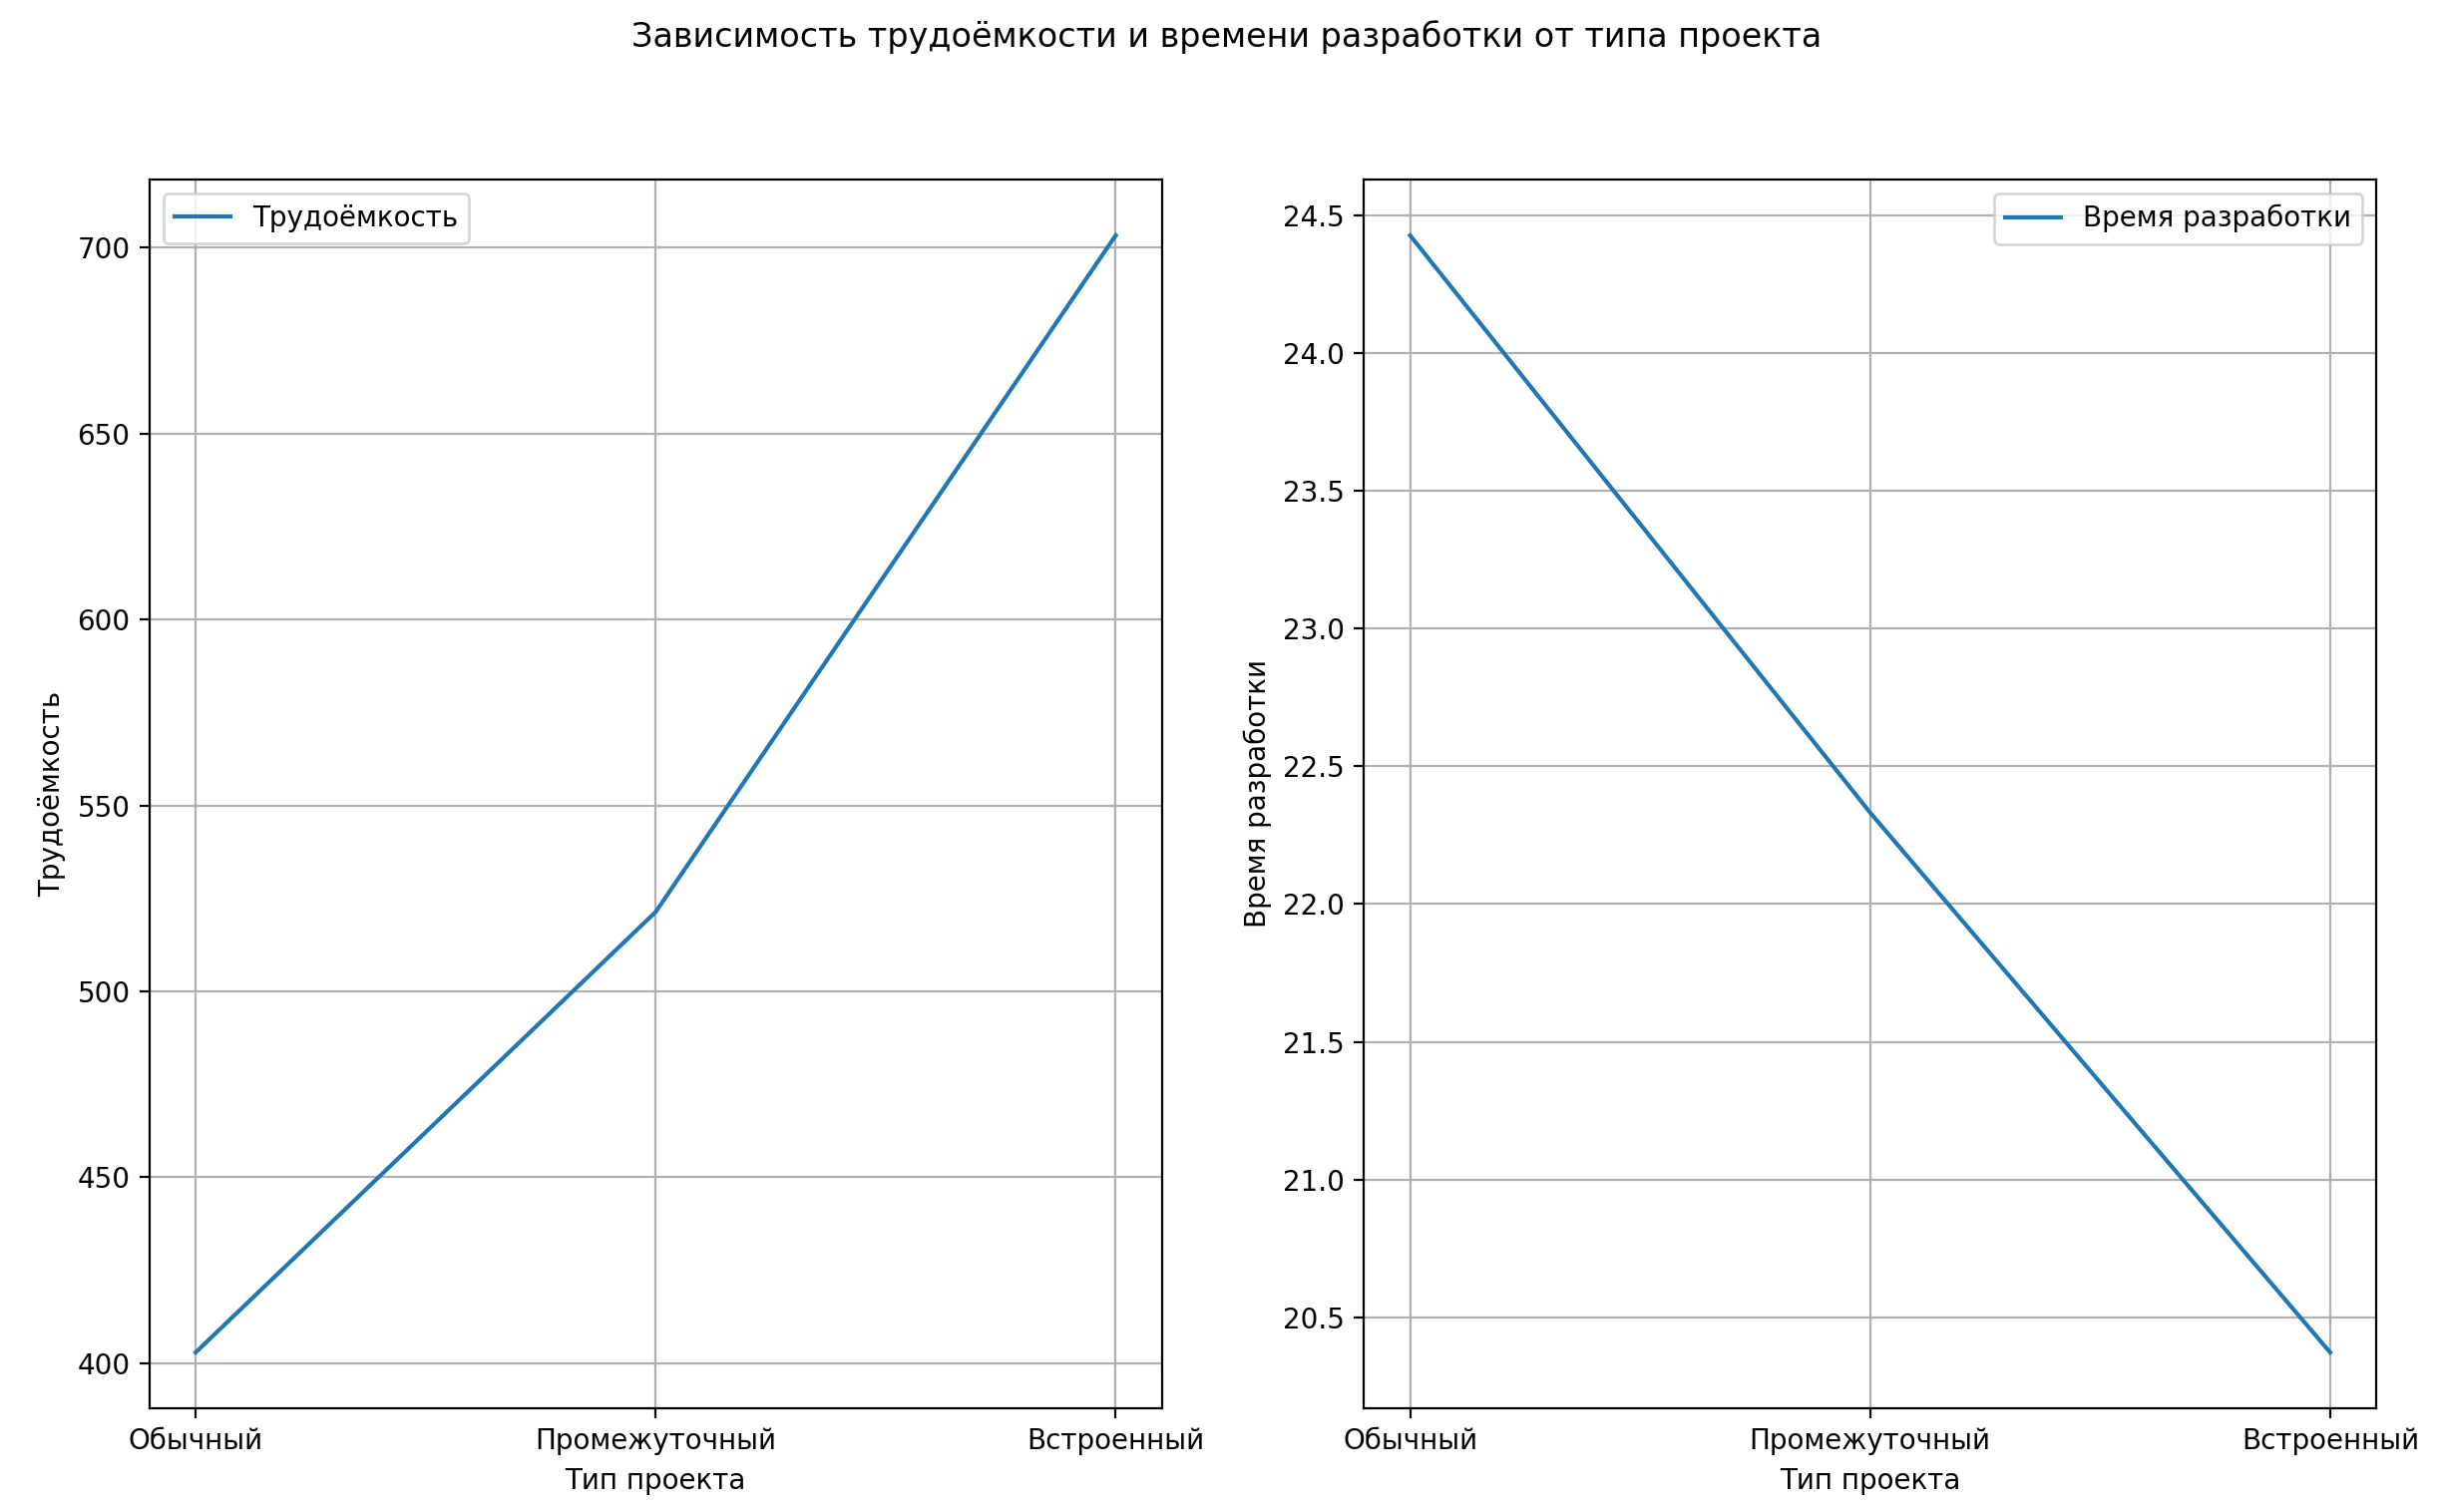
\includegraphics[scale=0.4, center]{lab06_task1_1}
\end{figure}

Из найденной зависимости следует, что с увеличением сложности проекта (от обычного к встроеннму) трудоёмкость проекта увеличивается, а время разработки уменьшается (обе зависимости почти линейны для фиксированного размера проекта в KLOC).

Отобразим зависимость влияния на трудоёмкость и время разработки уровня способностей ключевых членов команды --- программиста и аналитика, а также влияние  параметров среды, таких, как использование современных методов и программных инструментов.
.
\clearpage

\begin{figure}[h!]
	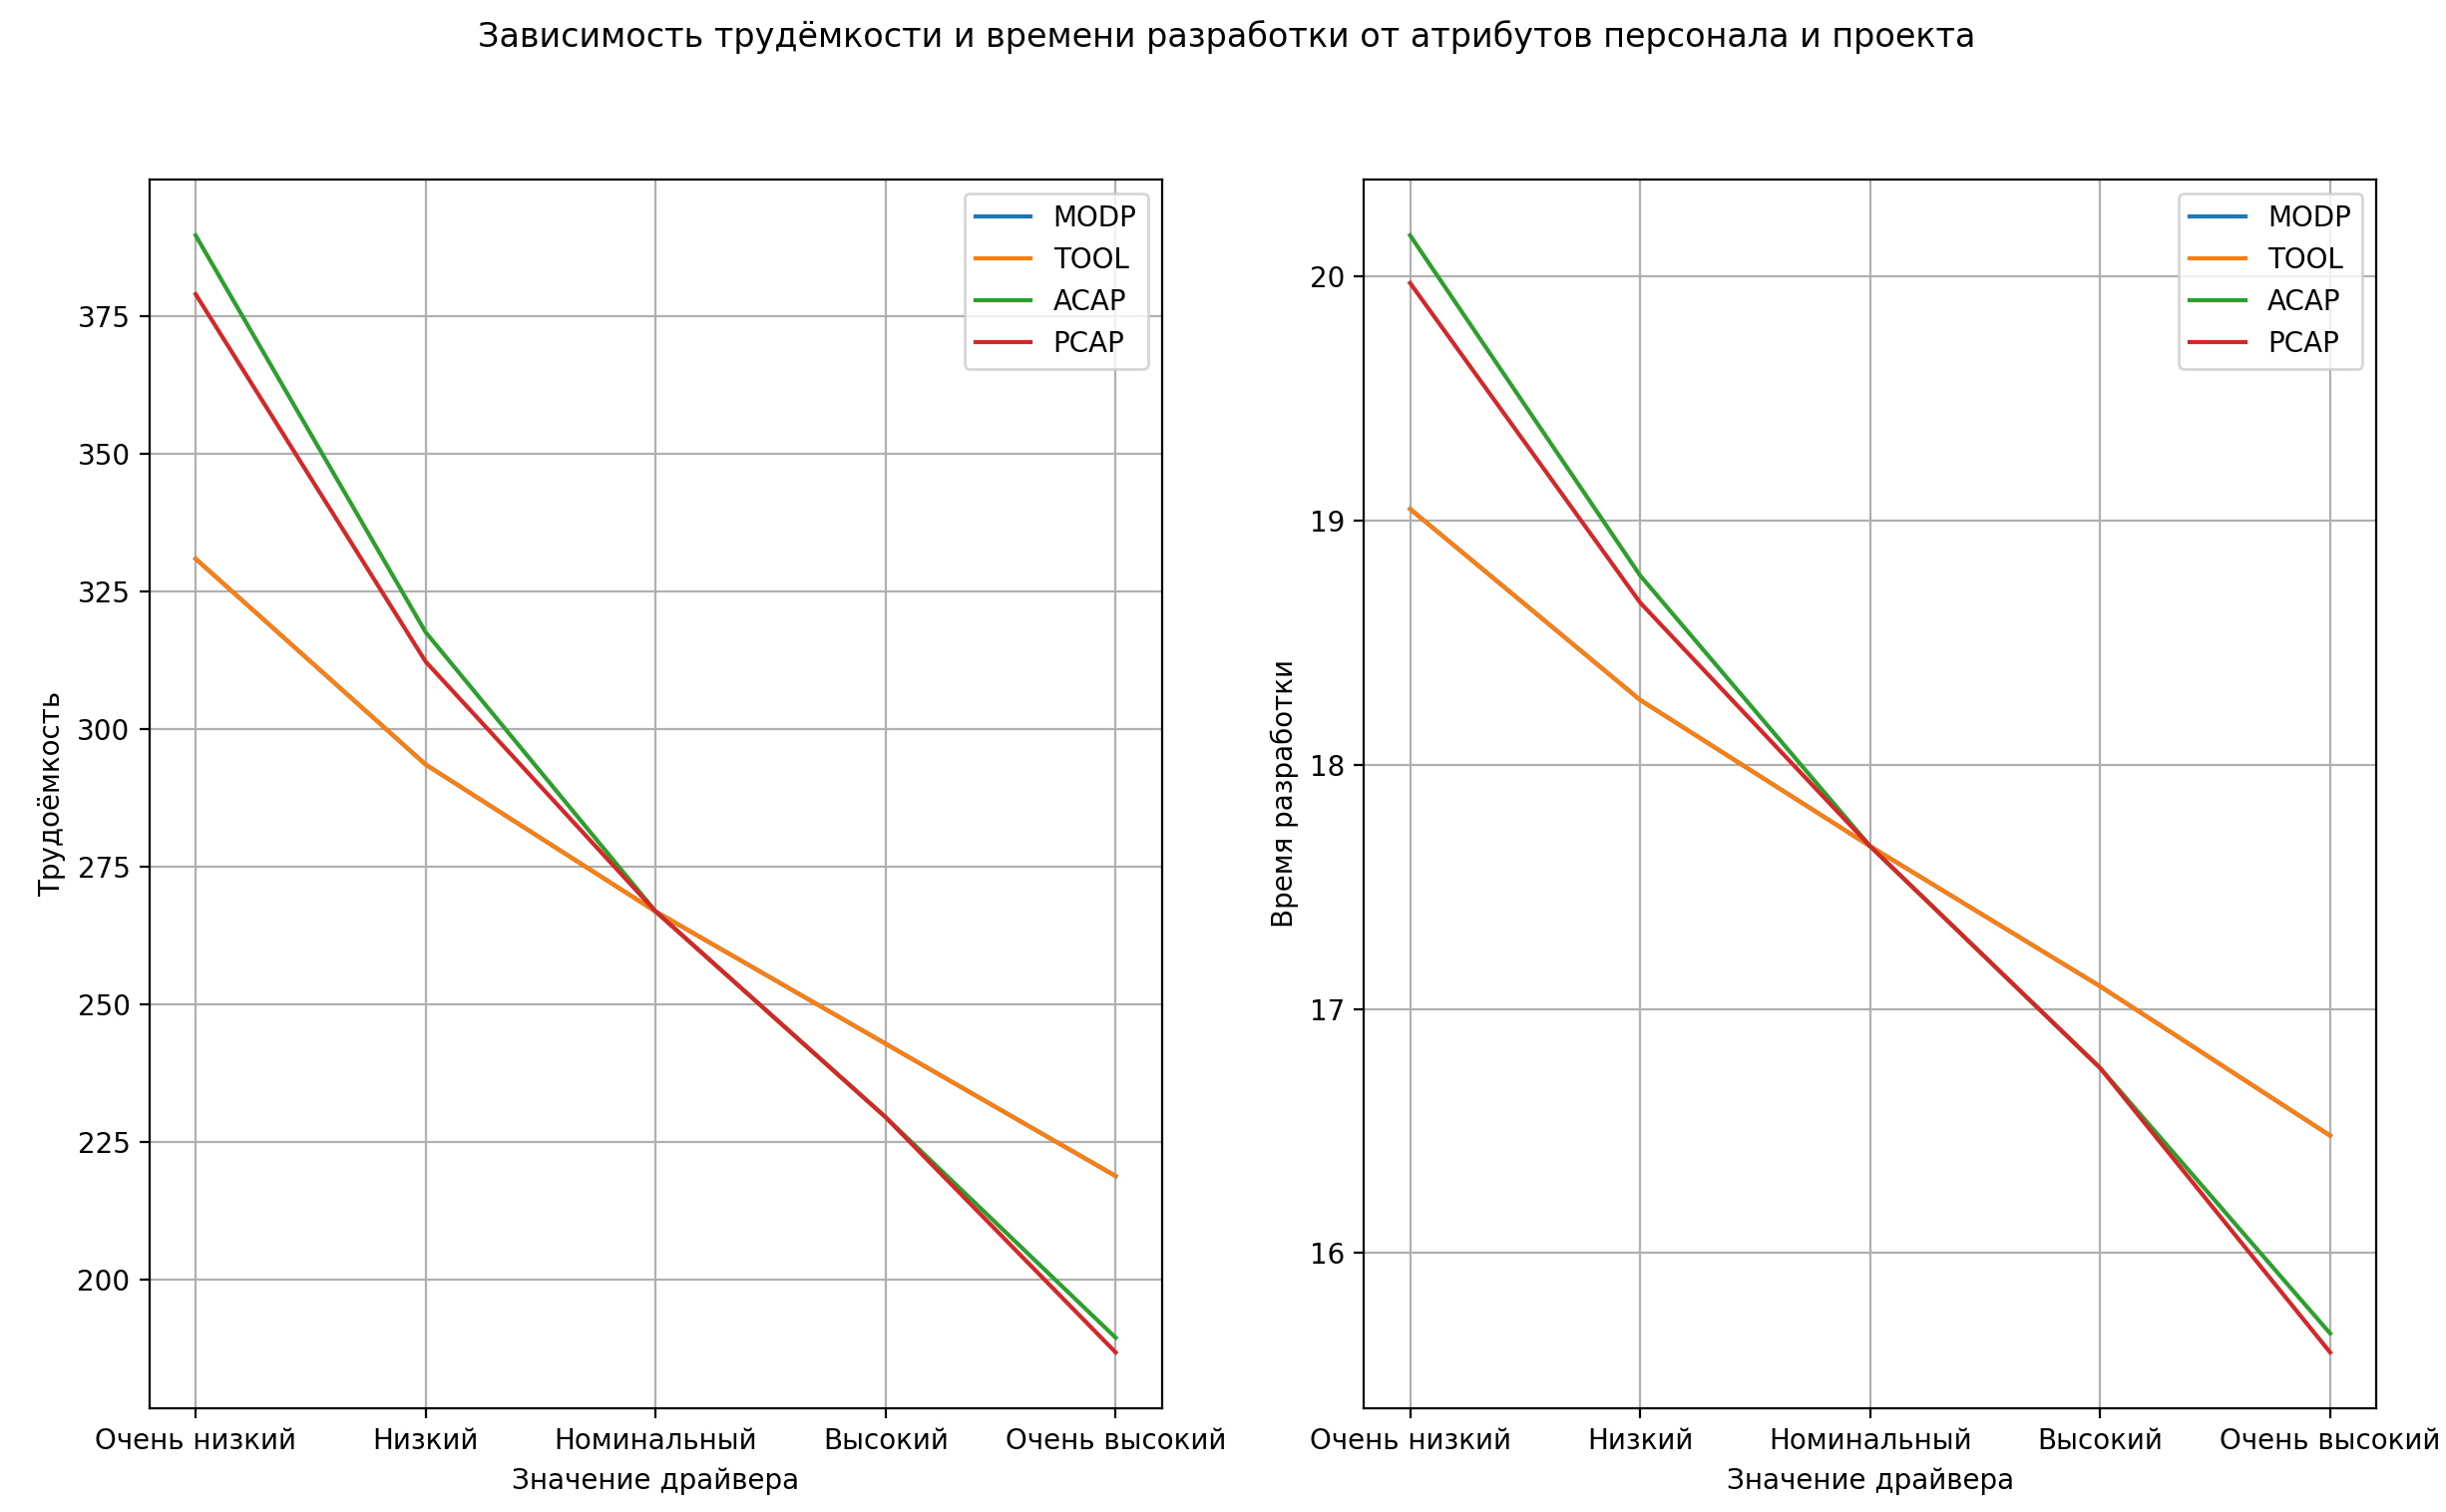
\includegraphics[scale=0.4, center]{lab06_task1_2}
\end{figure}

Из отображённой зависимости следует, что с использование современных методов и проограммных инструментов трудоёмкость и время разработки существенно (почти линейно) уменьшается, при этом атрибуты персонала влияют на трудоёмкость и время разработки больше, чем атрибуты проекта. 

Умения аналитика влияют на трудоёмкость и время разработки больше, чем умения програмиста, а влияние современных методов является почти таким же, как и влияние программных инструментов. При необходимости сократить срок выполнения проекта больше повлияют способности персонала.

\subsection*{Задание 2}

\subsubsection{Условие задания}

Компания получила заказ на разработку программного обеспечения для рабочей станции дизайнера автомобиля. 
Заказчик следующим образом определил проблемную область в своей спецификации: ПО должно формировать 2-х и 3-х мерные изображения для дизайнера, система должна иметь стандартизованный графический интерфейс, геометрические и прикладные данные должны содержаться в базе данных, планируемый размер которой не более 200 тыс. записей. При анализе проекта его размер был предварительно оценен в 140 000 строк кода. 
Проект реализуется по промежуточному варианту. 
Все  показатели драйверов затрат, кроме трех имеют номинальное значение: знание языка программирования имеет высокую оценку, использование современных методов – очень высокую оценку и использование программных инструментов – низкую, так как используется стандартная среда визуального программирования.
Произвести оценку показателей проекта по методике СОСОМО. 

\subsubsection{Выполнение}

При помощи разработанного калькулятора оценим показатели проекта по методике COCOMO:

\begin{figure}[h!]
	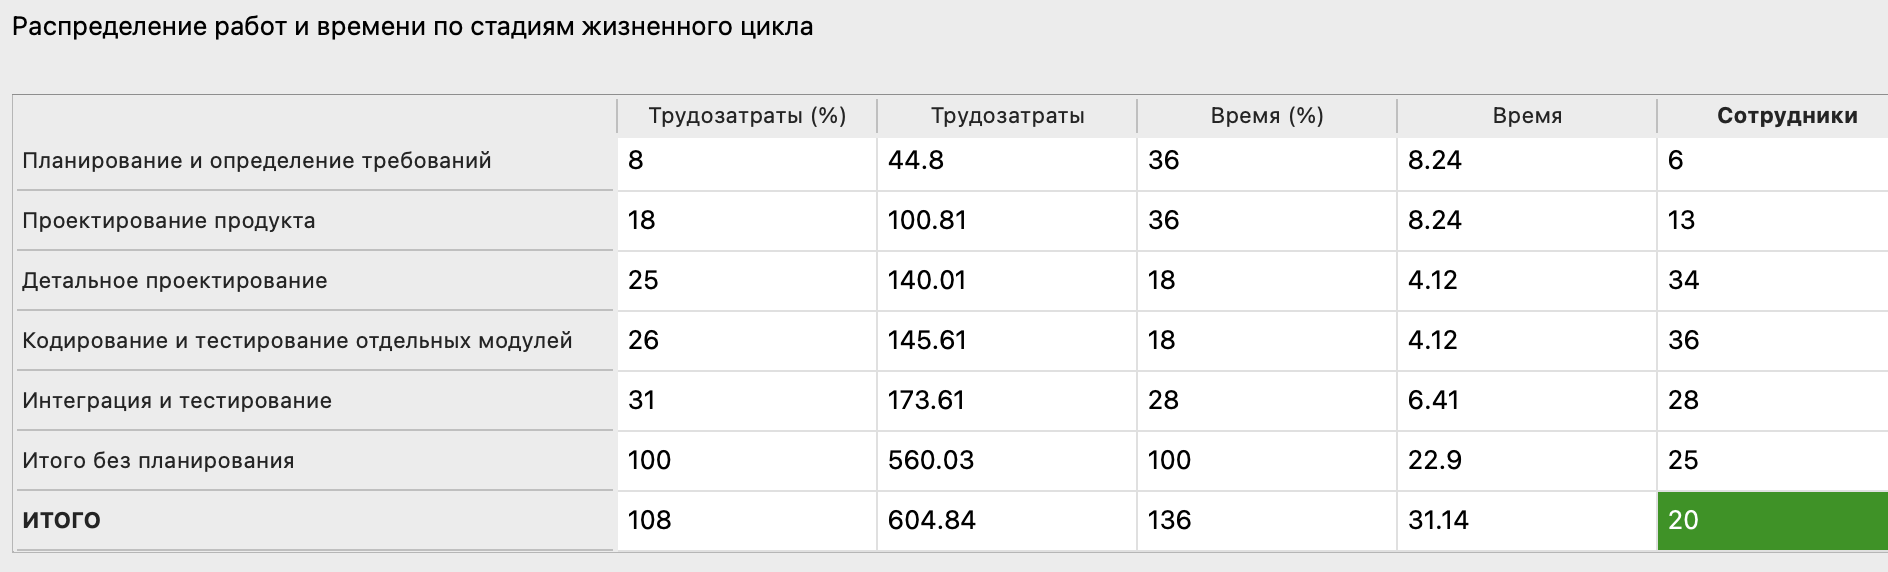
\includegraphics[scale=0.5, center]{lab06_task2_1}
\end{figure}

Трудозатраты (без учёта планирования и определения требований) составили 560 человеко-месяцев, время --- 23 месяца.

Требуемое для конкретного этапа выполнения проекта число сотрудников вычисляется следующим образом:

\begin{equation}
	\text{Число} = \frac{\text{Трудозатраты}}{\text{Время}}.
\end{equation}

Отобразим диаграмму привлечения сотрудников, причём 

\begin{itemize}
	\item A --- планирование и определение требований;
	\item B --- проектирование продукта;
	\item C --- детальное проектирование;
	\item D --- кодирование и тестирование отдельных модулей;
	\item E --- интеграция и тестирование.
\end{itemize}

\begin{figure}[h!]
	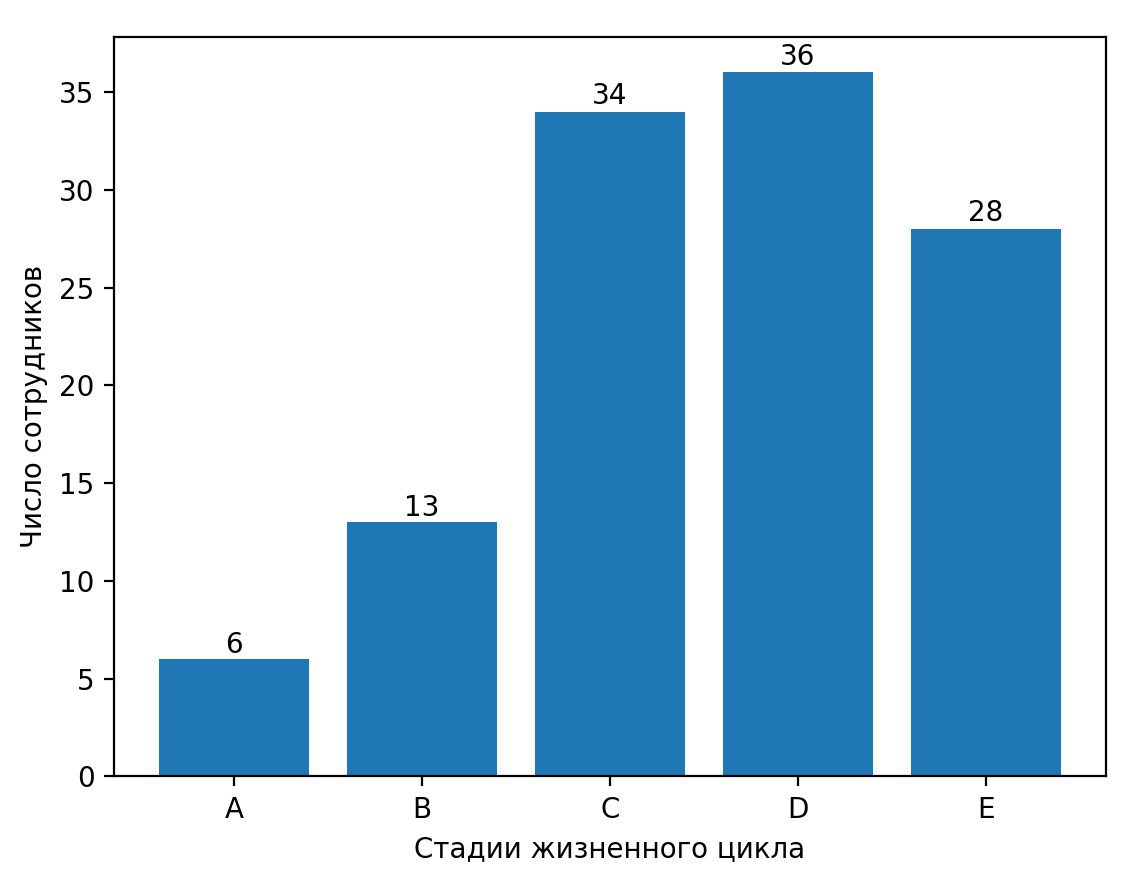
\includegraphics[scale=0.5, center]{lab06_task2_2}
\end{figure}

Предварительную оценку бюджета проекта можно определить так:

\begin{equation}
	\text{Бюджет} = \text{Трудозатраты}\cdot\text{Средняя заработная плата}.
\end{equation}

Отобразим распределение работ по видам деятельности WBS:
\begin{figure}[h!]
	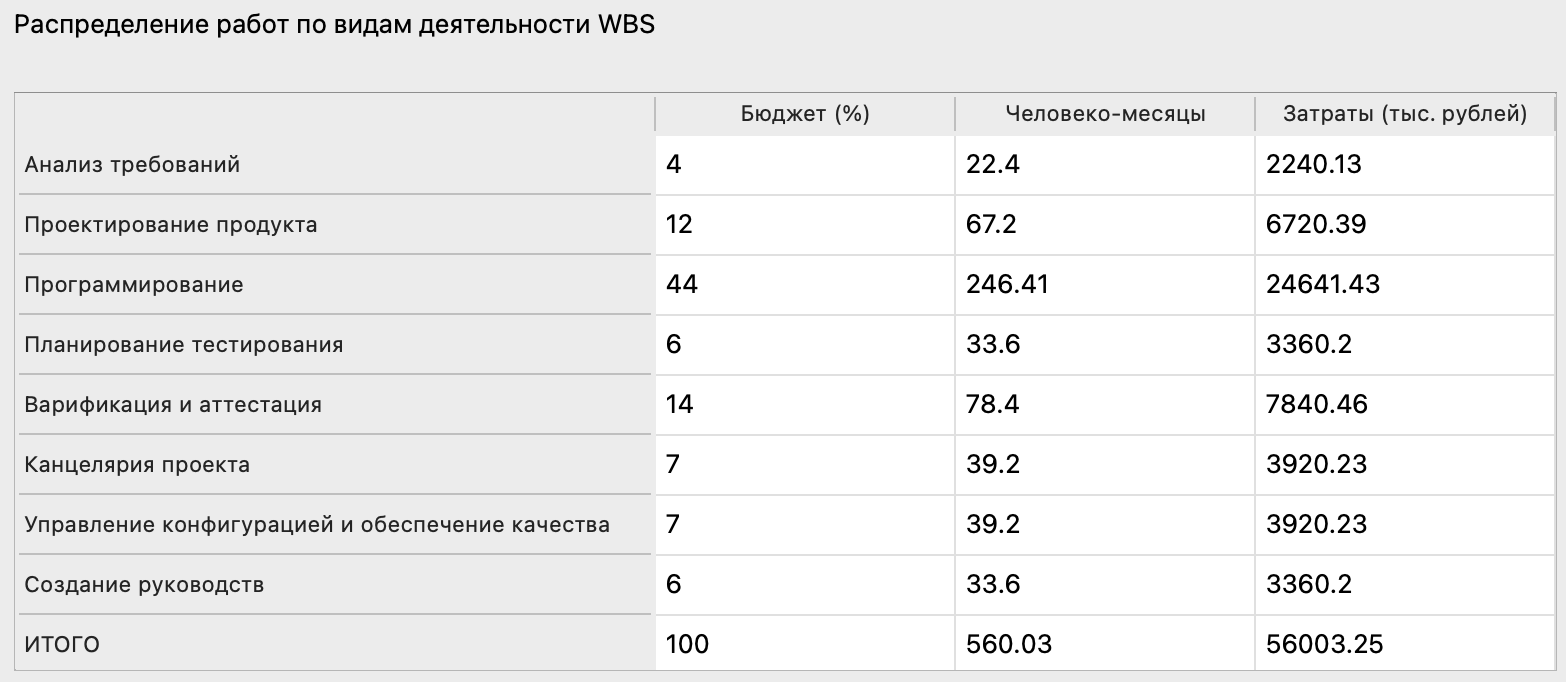
\includegraphics[scale=0.5, center]{lab06_task2_3}
\end{figure}

Для средней заработной платы 100 000 рублей проект обойдется примерно в 56 миллионов рублей, трудозатраты без учёта планирования и определения требований составят 560 человеко-месяцев, (а с их учётом --- 604), наибольшие затраты (24 миллиона рублей) приходятся на прграммирование, а наибольшее число сотрудников (36) нужно на кодирование и тестирование отдельных модулей. 

\section*{Заключение}

При выполнении лабораторной работы были отработаны навыки предварительной оценки параметров программного проекта на примере методики COCOMO.

С использованием модели COCOMO можно выполнить предварительную оценку трудозатрат, длительности выполнения и стоимости проекта. При этом методика позволяет производить расчеты для проектов разных масштабов с учетом их индивидуальных характеристик и проста в применении. 

К недостаткам методики COCOMO можно отнести следующее: расчеты в модели зависят от размера проекта, поэтому точность оценки проекта зависит от точности оценки размера. Не учитывается повторное использование компонентов, что влияет на размер проекта. Также методика COCOMO основана на каскадной модели жизненного цикла, поэтому не учитывает тонкости других методологий.
